\documentclass[a4paper]{book}
\usepackage{a4wide}
\usepackage{makeidx}
\usepackage{graphicx}
\usepackage{multicol}
\usepackage{float}
\usepackage{listings}
\usepackage{color}
\usepackage{textcomp}
\usepackage{alltt}
\usepackage{times}
\usepackage{ifpdf}
\ifpdf
\usepackage[pdftex,
            pagebackref=true,
            colorlinks=true,
            linkcolor=blue,
            unicode
           ]{hyperref}
\else
\usepackage[ps2pdf,
            pagebackref=true,
            colorlinks=true,
            linkcolor=blue,
            unicode
           ]{hyperref}
\usepackage{pspicture}
\fi
\usepackage[utf8]{inputenc}
\usepackage{doxygen}
\lstset{language=C++,inputencoding=utf8,basicstyle=\footnotesize,breaklines=true,breakatwhitespace=true,tabsize=8,numbers=left }
\makeindex
\setcounter{tocdepth}{3}
\renewcommand{\footrulewidth}{0.4pt}
\begin{document}
\hypersetup{pageanchor=false}
\begin{titlepage}
\vspace*{7cm}
\begin{center}
{\Large LittleBenchmark\_\-HDD \\[1ex]\large 0.10.6 }\\
\vspace*{1cm}
{\large Generated by Doxygen 1.6.3}\\
\vspace*{0.5cm}
{\small Sun Oct 10 13:35:42 2010}\\
\end{center}
\end{titlepage}
\clearemptydoublepage
\pagenumbering{roman}
\tableofcontents
\clearemptydoublepage
\pagenumbering{arabic}
\hypersetup{pageanchor=true}
\chapter{Class Index}
\section{Class Hierarchy}
This inheritance list is sorted roughly, but not completely, alphabetically:\begin{DoxyCompactList}
\item \contentsline{section}{profileUpdateStore}{\pageref{classprofileUpdateStore}}{}
\item \contentsline{section}{tester\_\-hdd}{\pageref{classtester__hdd}}{}
\item \contentsline{section}{myThreadTemplates::thread\_\-1$<$ ClassT $>$}{\pageref{classmyThreadTemplates_1_1thread__1}}{}
\item \contentsline{section}{myThreadTemplates::thread\_\-1$<$ thread\_\-tester\_\-hdd $>$}{\pageref{classmyThreadTemplates_1_1thread__1}}{}
\begin{DoxyCompactList}
\item \contentsline{section}{thread\_\-tester\_\-hdd}{\pageref{classthread__tester__hdd}}{}
\end{DoxyCompactList}
\end{DoxyCompactList}

\chapter{Class Index}
\section{Class List}
Here are the classes, structs, unions and interfaces with brief descriptions:\begin{DoxyCompactList}
\item\contentsline{section}{\hyperlink{classprofileUpdateStore}{profileUpdateStore} }{\pageref{classprofileUpdateStore}}{}
\item\contentsline{section}{\hyperlink{classstats__keeper}{stats\_\-keeper} }{\pageref{classstats__keeper}}{}
\item\contentsline{section}{\hyperlink{classtester__hdd}{tester\_\-hdd} }{\pageref{classtester__hdd}}{}
\item\contentsline{section}{\hyperlink{classmyThreadTemplates_1_1thread__1}{myThreadTemplates::thread\_\-1$<$ ClassT $>$} (Thread\_\-1 is very simple thread template which constainst few controle methods and entry for statistics )}{\pageref{classmyThreadTemplates_1_1thread__1}}{}
\item\contentsline{section}{\hyperlink{classthread__tester__hdd}{thread\_\-tester\_\-hdd$<$ classT $>$} }{\pageref{classthread__tester__hdd}}{}
\item\contentsline{section}{\hyperlink{structvector__str}{vector\_\-str} }{\pageref{structvector__str}}{}
\end{DoxyCompactList}

\chapter{Class Documentation}
\hypertarget{classhandler__Configuration}{
\section{handler\_\-Configuration Class Reference}
\label{classhandler__Configuration}\index{handler\_\-Configuration@{handler\_\-Configuration}}
}
Inheritance diagram for handler\_\-Configuration:\begin{figure}[H]
\begin{center}
\leavevmode
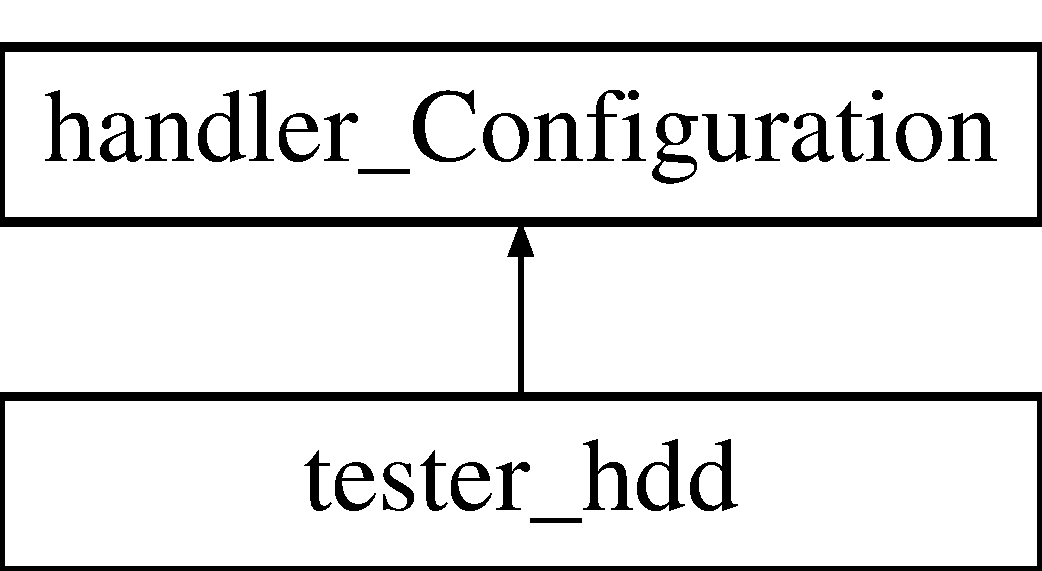
\includegraphics[height=2cm]{classhandler__Configuration}
\end{center}
\end{figure}
\subsection*{Public Member Functions}
\begin{DoxyCompactItemize}
\item 
void \hyperlink{classhandler__Configuration_a9f850565461949dbb96f6cc5028618c1}{setUserDir} ()
\item 
\hypertarget{classhandler__Configuration_a0dcef9ff84f43679905f5e5c81f5653f}{
void {\bfseries addNodeToStored} (string, string)}
\label{classhandler__Configuration_a0dcef9ff84f43679905f5e5c81f5653f}

\item 
\hypertarget{classhandler__Configuration_abcaa51f67c80dce0b76a9fee5c19b59a}{
void {\bfseries clearNodes} ()}
\label{classhandler__Configuration_abcaa51f67c80dce0b76a9fee5c19b59a}

\item 
\hypertarget{classhandler__Configuration_a3dc84c5be06ae0caa5c53954842e407f}{
void {\bfseries parseConfigs} ()}
\label{classhandler__Configuration_a3dc84c5be06ae0caa5c53954842e407f}

\item 
\hypertarget{classhandler__Configuration_ab7b078c0151a3c1efba8d2079cefcce8}{
void {\bfseries saveConfigs} ()}
\label{classhandler__Configuration_ab7b078c0151a3c1efba8d2079cefcce8}

\end{DoxyCompactItemize}
\subsection*{Protected Attributes}
\begin{DoxyCompactItemize}
\item 
\hypertarget{classhandler__Configuration_aa4302de200eb462a44938b64cb7ed944}{
boost::filesystem::path \hyperlink{classhandler__Configuration_aa4302de200eb462a44938b64cb7ed944}{pathProfile}}
\label{classhandler__Configuration_aa4302de200eb462a44938b64cb7ed944}

\begin{DoxyCompactList}\small\item\em Keeps path to config file. \item\end{DoxyCompactList}\item 
\hypertarget{classhandler__Configuration_af547a16146ccb86cf5102068e855b3a2}{
boost::filesystem::path \hyperlink{classhandler__Configuration_af547a16146ccb86cf5102068e855b3a2}{pathConfig}}
\label{classhandler__Configuration_af547a16146ccb86cf5102068e855b3a2}

\begin{DoxyCompactList}\small\item\em Keeps path to config file. \item\end{DoxyCompactList}\item 
\hypertarget{classhandler__Configuration_a1227b6391e07475da9686931a66b8150}{
bool {\bfseries bLetUpdate}}
\label{classhandler__Configuration_a1227b6391e07475da9686931a66b8150}

\end{DoxyCompactItemize}


\subsection{Member Function Documentation}
\hypertarget{classhandler__Configuration_a9f850565461949dbb96f6cc5028618c1}{
\index{handler\_\-Configuration@{handler\_\-Configuration}!setUserDir@{setUserDir}}
\index{setUserDir@{setUserDir}!handler_Configuration@{handler\_\-Configuration}}
\subsubsection[{setUserDir}]{\setlength{\rightskip}{0pt plus 5cm}void handler\_\-Configuration::setUserDir ()}}
\label{classhandler__Configuration_a9f850565461949dbb96f6cc5028618c1}


Creates program profile directory for current user 



The documentation for this class was generated from the following files:\begin{DoxyCompactItemize}
\item 
handler\_\-Configuration.hpp\item 
handler\_\-Configuration.cpp\end{DoxyCompactItemize}

\hypertarget{classhandler__Report}{
\section{handler\_\-Report Class Reference}
\label{classhandler__Report}\index{handler\_\-Report@{handler\_\-Report}}
}
Inheritance diagram for handler\_\-Report:\begin{figure}[H]
\begin{center}
\leavevmode
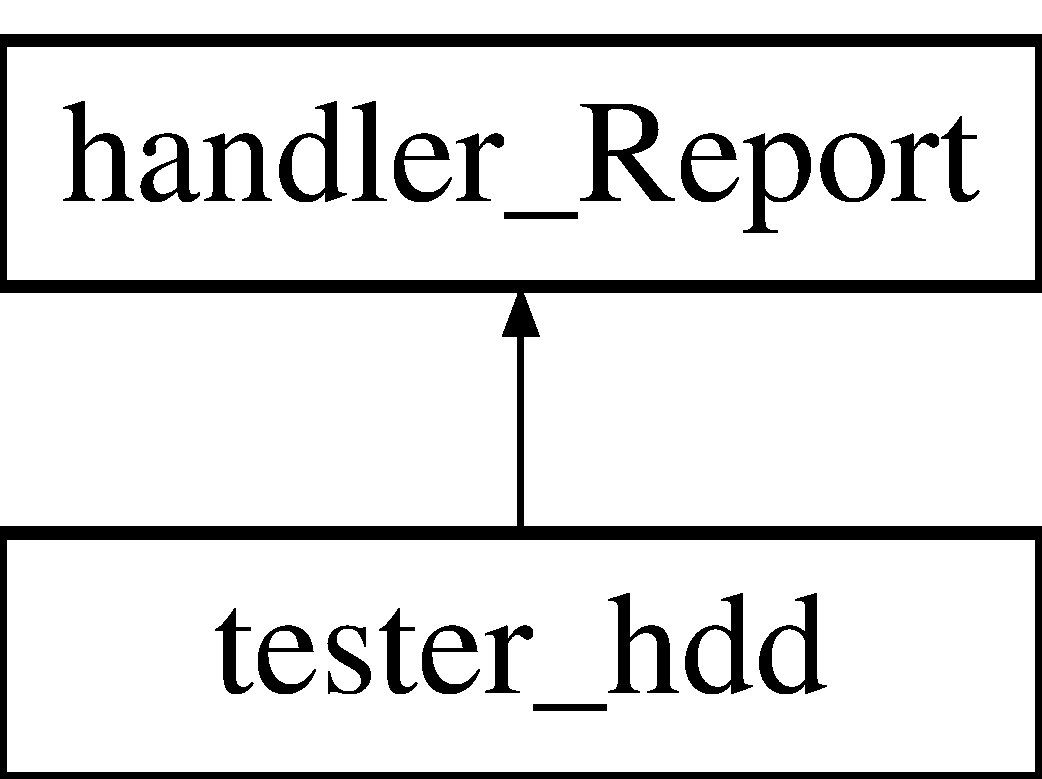
\includegraphics[height=2cm]{classhandler__Report}
\end{center}
\end{figure}
\subsection*{Public Member Functions}
\begin{DoxyCompactItemize}
\item 
\hypertarget{classhandler__Report_a69a82b65c02449796be662b897ee56fc}{
\hyperlink{classhandler__Report_a69a82b65c02449796be662b897ee56fc}{handler\_\-Report} ()}
\label{classhandler__Report_a69a82b65c02449796be662b897ee56fc}

\begin{DoxyCompactList}\small\item\em Constractor set all args with default values. \item\end{DoxyCompactList}\item 
\hypertarget{classhandler__Report_ae03757935a7d0ee9a4b1a8ef15b54040}{
void \hyperlink{classhandler__Report_ae03757935a7d0ee9a4b1a8ef15b54040}{addStatData} (string \&, string \&, unsigned=1, unsigned=1)}
\label{classhandler__Report_ae03757935a7d0ee9a4b1a8ef15b54040}

\begin{DoxyCompactList}\small\item\em Will add data to specified buffers. \item\end{DoxyCompactList}\item 
\hypertarget{classhandler__Report_af493d5f27da28ae1f611315208a98b83}{
uint8\_\-t {\bfseries findAndAdd} (string \&, string \&, unsigned=1, unsigned=1)}
\label{classhandler__Report_af493d5f27da28ae1f611315208a98b83}

\item 
\hypertarget{classhandler__Report_a56de9bfebe51073d5d85d0660418cd06}{
void {\bfseries FormatDataInVector} ()}
\label{classhandler__Report_a56de9bfebe51073d5d85d0660418cd06}

\item 
\hypertarget{classhandler__Report_a566af7550041c738548f29da0fd4a9ea}{
void {\bfseries SaveToDisk} (boost::filesystem::path)}
\label{classhandler__Report_a566af7550041c738548f29da0fd4a9ea}

\item 
\hypertarget{classhandler__Report_ab389a775c2650f0a5954be52c9a362a3}{
string \hyperlink{classhandler__Report_ab389a775c2650f0a5954be52c9a362a3}{GeneratDataFromVector} ()}
\label{classhandler__Report_ab389a775c2650f0a5954be52c9a362a3}

\begin{DoxyCompactList}\small\item\em Return refernce to string value generated from vector. \item\end{DoxyCompactList}\item 
\hypertarget{classhandler__Report_ae9889e1bb0a6a23d35a7a513a2f4056f}{
string {\bfseries GenerateXMLFromVector} ()}
\label{classhandler__Report_ae9889e1bb0a6a23d35a7a513a2f4056f}

\end{DoxyCompactItemize}
\subsection*{Protected Member Functions}
\begin{DoxyCompactItemize}
\item 
\hypertarget{classhandler__Report_a1406730673c2d437877e0f76ed5901f4}{
void \hyperlink{classhandler__Report_a1406730673c2d437877e0f76ed5901f4}{setArgs} ()}
\label{classhandler__Report_a1406730673c2d437877e0f76ed5901f4}

\begin{DoxyCompactList}\small\item\em Set Args determinates functionality. \item\end{DoxyCompactList}\end{DoxyCompactItemize}
\subsection*{Protected Attributes}
\begin{DoxyCompactItemize}
\item 
\hypertarget{classhandler__Report_a2a2e8a8bc459a3b007acb40ff556c2ae}{
vector$<$ string $>$ $\ast$ \hyperlink{classhandler__Report_a2a2e8a8bc459a3b007acb40ff556c2ae}{p\_\-vecstr\_\-Log}}
\label{classhandler__Report_a2a2e8a8bc459a3b007acb40ff556c2ae}

\begin{DoxyCompactList}\small\item\em keep log output in vector \item\end{DoxyCompactList}\item 
\hypertarget{classhandler__Report_aa36af55735b04c6bcc41a27fc913caff}{
vector$<$ \hyperlink{structstructRow}{structRow} $>$ $\ast$ \hyperlink{classhandler__Report_aa36af55735b04c6bcc41a27fc913caff}{p\_\-vecstr\_\-formattedTXT}}
\label{classhandler__Report_aa36af55735b04c6bcc41a27fc913caff}

\begin{DoxyCompactList}\small\item\em keep data in vector \item\end{DoxyCompactList}\item 
\hypertarget{classhandler__Report_a9837a9440d4966101ce058aac3d9f2c1}{
boost::filesystem::path \hyperlink{classhandler__Report_a9837a9440d4966101ce058aac3d9f2c1}{pathReport}}
\label{classhandler__Report_a9837a9440d4966101ce058aac3d9f2c1}

\begin{DoxyCompactList}\small\item\em Keeps path to report file. \item\end{DoxyCompactList}\item 
\hypertarget{classhandler__Report_a3886bbd9c74f29d506556d9e5df880b3}{
string \hyperlink{classhandler__Report_a3886bbd9c74f29d506556d9e5df880b3}{strReportFile}}
\label{classhandler__Report_a3886bbd9c74f29d506556d9e5df880b3}

\begin{DoxyCompactList}\small\item\em File to report will be written. \item\end{DoxyCompactList}\item 
\hypertarget{classhandler__Report_a31a53042cd0a7573c6085f873cc7c9c2}{
bool \hyperlink{classhandler__Report_a31a53042cd0a7573c6085f873cc7c9c2}{bLog}}
\label{classhandler__Report_a31a53042cd0a7573c6085f873cc7c9c2}

\begin{DoxyCompactList}\small\item\em To log. \item\end{DoxyCompactList}\item 
\hypertarget{classhandler__Report_a01b617c244828e8b335d340c7100cda9}{
bool \hyperlink{classhandler__Report_a01b617c244828e8b335d340c7100cda9}{bFormattedTxt}}
\label{classhandler__Report_a01b617c244828e8b335d340c7100cda9}

\begin{DoxyCompactList}\small\item\em Generate formatted txt. \item\end{DoxyCompactList}\item 
\hypertarget{classhandler__Report_af4d0a63e01b33543e5c99f506e26b501}{
bool \hyperlink{classhandler__Report_af4d0a63e01b33543e5c99f506e26b501}{bGenXML}}
\label{classhandler__Report_af4d0a63e01b33543e5c99f506e26b501}

\begin{DoxyCompactList}\small\item\em Generate xml. \item\end{DoxyCompactList}\item 
\hypertarget{classhandler__Report_a4c432f8d94b302551fc555c5ecc38be3}{
unsigned \hyperlink{classhandler__Report_a4c432f8d94b302551fc555c5ecc38be3}{uiMultiplySpacer}}
\label{classhandler__Report_a4c432f8d94b302551fc555c5ecc38be3}

\begin{DoxyCompactList}\small\item\em Multiply spacer. \item\end{DoxyCompactList}\item 
\hypertarget{classhandler__Report_abe60637871a948045fc0c8a9bf55a096}{
unsigned \hyperlink{classhandler__Report_abe60637871a948045fc0c8a9bf55a096}{uiMaxCols}}
\label{classhandler__Report_abe60637871a948045fc0c8a9bf55a096}

\begin{DoxyCompactList}\small\item\em Max columns. \item\end{DoxyCompactList}\item 
\hypertarget{classhandler__Report_a3ab81c5a6cdd06611c7e2e6d2d2424e3}{
string \hyperlink{classhandler__Report_a3ab81c5a6cdd06611c7e2e6d2d2424e3}{strSpacerChar}}
\label{classhandler__Report_a3ab81c5a6cdd06611c7e2e6d2d2424e3}

\begin{DoxyCompactList}\small\item\em spacer character \item\end{DoxyCompactList}\end{DoxyCompactItemize}


The documentation for this class was generated from the following files:\begin{DoxyCompactItemize}
\item 
handler\_\-Report.hpp\item 
handler\_\-Report.cpp\end{DoxyCompactItemize}

\hypertarget{structprofileNode}{
\section{profileNode Struct Reference}
\label{structprofileNode}\index{profileNode@{profileNode}}
}
\subsection*{Public Member Functions}
\begin{DoxyCompactItemize}
\item 
\hypertarget{structprofileNode_a406a027ccda90573940b1fd7dc019652}{
{\bfseries profileNode} (const string \&, const string \&)}
\label{structprofileNode_a406a027ccda90573940b1fd7dc019652}

\item 
\hypertarget{structprofileNode_aa2d5252dd9a7e41c78a43ebdf6cc3301}{
string {\bfseries getData} ()}
\label{structprofileNode_aa2d5252dd9a7e41c78a43ebdf6cc3301}

\end{DoxyCompactItemize}
\subsection*{Public Attributes}
\begin{DoxyCompactItemize}
\item 
\hypertarget{structprofileNode_a6b91777554bee2d799c90ea4f650490c}{
string {\bfseries strVar}}
\label{structprofileNode_a6b91777554bee2d799c90ea4f650490c}

\item 
\hypertarget{structprofileNode_a138f86b8e22541f1bf6a12dd361ac1bb}{
string {\bfseries strVal}}
\label{structprofileNode_a138f86b8e22541f1bf6a12dd361ac1bb}

\end{DoxyCompactItemize}


The documentation for this struct was generated from the following files:\begin{DoxyCompactItemize}
\item 
handler\_\-Configuration.hpp\item 
handler\_\-Configuration.cpp\end{DoxyCompactItemize}

\hypertarget{structstructRow}{
\section{structRow Struct Reference}
\label{structstructRow}\index{structRow@{structRow}}
}
\subsection*{Public Member Functions}
\begin{DoxyCompactItemize}
\item 
\hyperlink{structstructRow_a09213fb7bb170a682869db469718761e}{structRow} (unsigned \&)
\end{DoxyCompactItemize}
\subsection*{Public Attributes}
\begin{DoxyCompactItemize}
\item 
\hypertarget{structstructRow_a627f7dc245b2dd29b2c94e02f5347573}{
vector$<$ string $>$ \hyperlink{structstructRow_a627f7dc245b2dd29b2c94e02f5347573}{data}}
\label{structstructRow_a627f7dc245b2dd29b2c94e02f5347573}

\begin{DoxyCompactList}\small\item\em Row. \item\end{DoxyCompactList}\end{DoxyCompactItemize}


\subsection{Constructor \& Destructor Documentation}
\hypertarget{structstructRow_a09213fb7bb170a682869db469718761e}{
\index{structRow@{structRow}!structRow@{structRow}}
\index{structRow@{structRow}!structRow@{structRow}}
\subsubsection[{structRow}]{\setlength{\rightskip}{0pt plus 5cm}structRow::structRow (unsigned \& {\em col})}}
\label{structstructRow_a09213fb7bb170a682869db469718761e}


Creates defined number of columns 



The documentation for this struct was generated from the following files:\begin{DoxyCompactItemize}
\item 
handler\_\-Report.hpp\item 
handler\_\-Report.cpp\end{DoxyCompactItemize}

\hypertarget{classtester__hdd}{
\section{tester\_\-hdd Class Reference}
\label{classtester__hdd}\index{tester\_\-hdd@{tester\_\-hdd}}
}
Inheritance diagram for tester\_\-hdd:\begin{figure}[H]
\begin{center}
\leavevmode
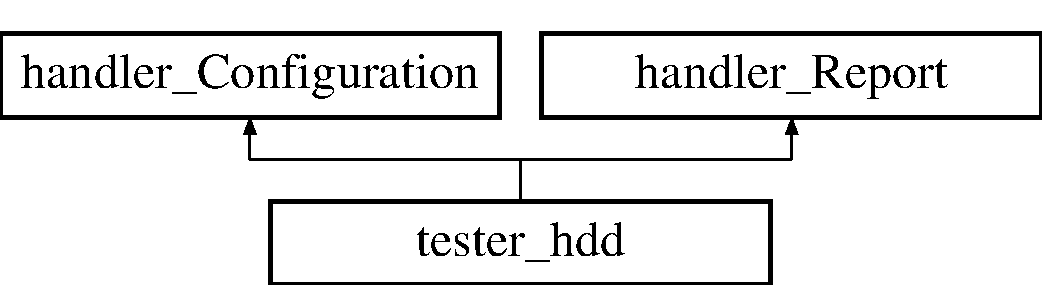
\includegraphics[height=2cm]{classtester__hdd}
\end{center}
\end{figure}
\subsection*{Public Member Functions}
\begin{DoxyCompactItemize}
\item 
\hyperlink{classtester__hdd_af43b8ca9595ed8ebf14b2c7cffe561c2}{tester\_\-hdd} (int, char $\ast$$\ast$)
\item 
void \hyperlink{classtester__hdd_abfdcc395e8be504dfd0ea686da790375}{Run} ()
\end{DoxyCompactItemize}
\subsection*{Public Attributes}
\begin{DoxyCompactItemize}
\item 
\hypertarget{classtester__hdd_a71413f3e5b1ecf13efe4eb8c9064a211}{
bool {\bfseries bRun}}
\label{classtester__hdd_a71413f3e5b1ecf13efe4eb8c9064a211}

\end{DoxyCompactItemize}


\subsection{Constructor \& Destructor Documentation}
\hypertarget{classtester__hdd_af43b8ca9595ed8ebf14b2c7cffe561c2}{
\index{tester\_\-hdd@{tester\_\-hdd}!tester\_\-hdd@{tester\_\-hdd}}
\index{tester\_\-hdd@{tester\_\-hdd}!tester_hdd@{tester\_\-hdd}}
\subsubsection[{tester\_\-hdd}]{\setlength{\rightskip}{0pt plus 5cm}tester\_\-hdd::tester\_\-hdd (int {\em ac}, \/  char $\ast$$\ast$ {\em av})}}
\label{classtester__hdd_af43b8ca9595ed8ebf14b2c7cffe561c2}
Important notes for Linux: $\ast$ In file /etc/nsswitch.conf change passwd compat to passwd file in order to prevent memory leak 

Creates user profile before parsing args

Number of columns

Set output args 



\subsection{Member Function Documentation}
\hypertarget{classtester__hdd_abfdcc395e8be504dfd0ea686da790375}{
\index{tester\_\-hdd@{tester\_\-hdd}!Run@{Run}}
\index{Run@{Run}!tester_hdd@{tester\_\-hdd}}
\subsubsection[{Run}]{\setlength{\rightskip}{0pt plus 5cm}void tester\_\-hdd::Run ()}}
\label{classtester__hdd_abfdcc395e8be504dfd0ea686da790375}


Create threads and insert it to list

Running threads from list

If multithreading is disable program will wait for thread to do its job before running next one

With multithreading wating for all started threads to end its jobs 



The documentation for this class was generated from the following files:\begin{DoxyCompactItemize}
\item 
tester\_\-hdd.hpp\item 
tester\_\-hdd.cpp\end{DoxyCompactItemize}

\hypertarget{classbuskol_1_1ThreadTemplates_1_1thread__1}{
\section{buskol::ThreadTemplates::thread\_\-1$<$ ClassT $>$ Class Template Reference}
\label{classbuskol_1_1ThreadTemplates_1_1thread__1}\index{buskol::ThreadTemplates::thread\_\-1@{buskol::ThreadTemplates::thread\_\-1}}
}


Thread\_\-1 is very simple thread template which constainst few controle methods and entry for statistics.  




{\ttfamily \#include $<$myThreadTemplates.hpp$>$}

\subsection*{Public Member Functions}
\begin{DoxyCompactItemize}
\item 
\hypertarget{classbuskol_1_1ThreadTemplates_1_1thread__1_abb320f878a938843b4d797300a2e4703}{
{\bfseries thread\_\-1} (ClassT $\ast$parent, list$<$ string $\ast$ $>$ $\ast$list=NULL, bool show=false)}
\label{classbuskol_1_1ThreadTemplates_1_1thread__1_abb320f878a938843b4d797300a2e4703}

\item 
void \hyperlink{classbuskol_1_1ThreadTemplates_1_1thread__1_a71250f676aa96d06d5b693b685af7555}{start} ()
\item 
void \hyperlink{classbuskol_1_1ThreadTemplates_1_1thread__1_ad3a839cb3ec07abf8cf54fe81fd5e7f3}{start\_\-self\_\-test} ()
\item 
void \hyperlink{classbuskol_1_1ThreadTemplates_1_1thread__1_af917523b30feb06614e96371a5c198ed}{join} ()
\item 
void \hyperlink{classbuskol_1_1ThreadTemplates_1_1thread__1_a7c62551333aad740fc7b48742cdeb877}{join} (unsigned val)
\item 
\hypertarget{classbuskol_1_1ThreadTemplates_1_1thread__1_a86326c7ac7bc204899f806510d9060e7}{
string {\bfseries GetThreadID} ()}
\label{classbuskol_1_1ThreadTemplates_1_1thread__1_a86326c7ac7bc204899f806510d9060e7}

\item 
void \hyperlink{classbuskol_1_1ThreadTemplates_1_1thread__1_ab97928f6c8b8c75b33ffd6e57514d692}{UpdateStats} (string $\ast$str)
\item 
virtual \hyperlink{classbuskol_1_1ThreadTemplates_1_1thread__1_a7e53c5d7bef0898efc1c1bb217c6319a}{$\sim$thread\_\-1} ()
\end{DoxyCompactItemize}
\subsection*{Static Public Member Functions}
\begin{DoxyCompactItemize}
\item 
static void \hyperlink{classbuskol_1_1ThreadTemplates_1_1thread__1_ac33a5aa33679452b203c539401c92929}{self\_\-test} ()
\item 
static void \hyperlink{classbuskol_1_1ThreadTemplates_1_1thread__1_a37cde0d5c6105d9194ce1cf981cf9c5a}{Execute\_\-} (ClassT $\ast$p)
\end{DoxyCompactItemize}


\subsection{Detailed Description}
\subsubsection*{template$<$class ClassT$>$ class buskol::ThreadTemplates::thread\_\-1$<$ ClassT $>$}

Thread\_\-1 is very simple thread template which constainst few controle methods and entry for statistics. 

\subsection{Constructor \& Destructor Documentation}
\hypertarget{classbuskol_1_1ThreadTemplates_1_1thread__1_a7e53c5d7bef0898efc1c1bb217c6319a}{
\index{buskol::ThreadTemplates::thread\_\-1@{buskol::ThreadTemplates::thread\_\-1}!$\sim$thread\_\-1@{$\sim$thread\_\-1}}
\index{$\sim$thread\_\-1@{$\sim$thread\_\-1}!buskol::ThreadTemplates::thread_1@{buskol::ThreadTemplates::thread\_\-1}}
\subsubsection[{$\sim$thread\_\-1}]{\setlength{\rightskip}{0pt plus 5cm}template$<$class ClassT$>$ virtual {\bf buskol::ThreadTemplates::thread\_\-1}$<$ ClassT $>$::$\sim${\bf thread\_\-1} ()\hspace{0.3cm}{\ttfamily  \mbox{[}inline, virtual\mbox{]}}}}
\label{classbuskol_1_1ThreadTemplates_1_1thread__1_a7e53c5d7bef0898efc1c1bb217c6319a}


Virtual destructor which can show time of execution 



\subsection{Member Function Documentation}
\hypertarget{classbuskol_1_1ThreadTemplates_1_1thread__1_a37cde0d5c6105d9194ce1cf981cf9c5a}{
\index{buskol::ThreadTemplates::thread\_\-1@{buskol::ThreadTemplates::thread\_\-1}!Execute\_\-@{Execute\_\-}}
\index{Execute\_\-@{Execute\_\-}!buskol::ThreadTemplates::thread_1@{buskol::ThreadTemplates::thread\_\-1}}
\subsubsection[{Execute\_\-}]{\setlength{\rightskip}{0pt plus 5cm}template$<$class ClassT$>$ static void {\bf buskol::ThreadTemplates::thread\_\-1}$<$ ClassT $>$::Execute\_\- (ClassT $\ast$ {\em p})\hspace{0.3cm}{\ttfamily  \mbox{[}inline, static\mbox{]}}}}
\label{classbuskol_1_1ThreadTemplates_1_1thread__1_a37cde0d5c6105d9194ce1cf981cf9c5a}


Static linker for dynamic method 

\hypertarget{classbuskol_1_1ThreadTemplates_1_1thread__1_a7c62551333aad740fc7b48742cdeb877}{
\index{buskol::ThreadTemplates::thread\_\-1@{buskol::ThreadTemplates::thread\_\-1}!join@{join}}
\index{join@{join}!buskol::ThreadTemplates::thread_1@{buskol::ThreadTemplates::thread\_\-1}}
\subsubsection[{join}]{\setlength{\rightskip}{0pt plus 5cm}template$<$class ClassT$>$ void {\bf buskol::ThreadTemplates::thread\_\-1}$<$ ClassT $>$::join (unsigned {\em val})\hspace{0.3cm}{\ttfamily  \mbox{[}inline\mbox{]}}}}
\label{classbuskol_1_1ThreadTemplates_1_1thread__1_a7c62551333aad740fc7b48742cdeb877}


Join thread after specified time in seconds 

\hypertarget{classbuskol_1_1ThreadTemplates_1_1thread__1_af917523b30feb06614e96371a5c198ed}{
\index{buskol::ThreadTemplates::thread\_\-1@{buskol::ThreadTemplates::thread\_\-1}!join@{join}}
\index{join@{join}!buskol::ThreadTemplates::thread_1@{buskol::ThreadTemplates::thread\_\-1}}
\subsubsection[{join}]{\setlength{\rightskip}{0pt plus 5cm}template$<$class ClassT$>$ void {\bf buskol::ThreadTemplates::thread\_\-1}$<$ ClassT $>$::join ()\hspace{0.3cm}{\ttfamily  \mbox{[}inline\mbox{]}}}}
\label{classbuskol_1_1ThreadTemplates_1_1thread__1_af917523b30feb06614e96371a5c198ed}


Join thread 

\hypertarget{classbuskol_1_1ThreadTemplates_1_1thread__1_ac33a5aa33679452b203c539401c92929}{
\index{buskol::ThreadTemplates::thread\_\-1@{buskol::ThreadTemplates::thread\_\-1}!self\_\-test@{self\_\-test}}
\index{self\_\-test@{self\_\-test}!buskol::ThreadTemplates::thread_1@{buskol::ThreadTemplates::thread\_\-1}}
\subsubsection[{self\_\-test}]{\setlength{\rightskip}{0pt plus 5cm}template$<$class ClassT$>$ static void {\bf buskol::ThreadTemplates::thread\_\-1}$<$ ClassT $>$::self\_\-test ()\hspace{0.3cm}{\ttfamily  \mbox{[}inline, static\mbox{]}}}}
\label{classbuskol_1_1ThreadTemplates_1_1thread__1_ac33a5aa33679452b203c539401c92929}


This method is only for test purpose! 

\hypertarget{classbuskol_1_1ThreadTemplates_1_1thread__1_a71250f676aa96d06d5b693b685af7555}{
\index{buskol::ThreadTemplates::thread\_\-1@{buskol::ThreadTemplates::thread\_\-1}!start@{start}}
\index{start@{start}!buskol::ThreadTemplates::thread_1@{buskol::ThreadTemplates::thread\_\-1}}
\subsubsection[{start}]{\setlength{\rightskip}{0pt plus 5cm}template$<$class ClassT$>$ void {\bf buskol::ThreadTemplates::thread\_\-1}$<$ ClassT $>$::start ()\hspace{0.3cm}{\ttfamily  \mbox{[}inline\mbox{]}}}}
\label{classbuskol_1_1ThreadTemplates_1_1thread__1_a71250f676aa96d06d5b693b685af7555}


Creates Thread and links it dynamic using static method 

\hypertarget{classbuskol_1_1ThreadTemplates_1_1thread__1_ad3a839cb3ec07abf8cf54fe81fd5e7f3}{
\index{buskol::ThreadTemplates::thread\_\-1@{buskol::ThreadTemplates::thread\_\-1}!start\_\-self\_\-test@{start\_\-self\_\-test}}
\index{start\_\-self\_\-test@{start\_\-self\_\-test}!buskol::ThreadTemplates::thread_1@{buskol::ThreadTemplates::thread\_\-1}}
\subsubsection[{start\_\-self\_\-test}]{\setlength{\rightskip}{0pt plus 5cm}template$<$class ClassT$>$ void {\bf buskol::ThreadTemplates::thread\_\-1}$<$ ClassT $>$::start\_\-self\_\-test ()\hspace{0.3cm}{\ttfamily  \mbox{[}inline\mbox{]}}}}
\label{classbuskol_1_1ThreadTemplates_1_1thread__1_ad3a839cb3ec07abf8cf54fe81fd5e7f3}


This method is only for test purpose! 

\hypertarget{classbuskol_1_1ThreadTemplates_1_1thread__1_ab97928f6c8b8c75b33ffd6e57514d692}{
\index{buskol::ThreadTemplates::thread\_\-1@{buskol::ThreadTemplates::thread\_\-1}!UpdateStats@{UpdateStats}}
\index{UpdateStats@{UpdateStats}!buskol::ThreadTemplates::thread_1@{buskol::ThreadTemplates::thread\_\-1}}
\subsubsection[{UpdateStats}]{\setlength{\rightskip}{0pt plus 5cm}template$<$class ClassT$>$ void {\bf buskol::ThreadTemplates::thread\_\-1}$<$ ClassT $>$::UpdateStats (string $\ast$ {\em str})\hspace{0.3cm}{\ttfamily  \mbox{[}inline\mbox{]}}}}
\label{classbuskol_1_1ThreadTemplates_1_1thread__1_ab97928f6c8b8c75b33ffd6e57514d692}


Push statistic information 



The documentation for this class was generated from the following file:\begin{DoxyCompactItemize}
\item 
myThreadTemplates.hpp\end{DoxyCompactItemize}

\hypertarget{classthread__tester__hdd}{
\section{thread\_\-tester\_\-hdd Class Reference}
\label{classthread__tester__hdd}\index{thread\_\-tester\_\-hdd@{thread\_\-tester\_\-hdd}}
}


Globals Varuabels.  




{\ttfamily \#include $<$thread\_\-tester\_\-hdd.hpp$>$}

Inheritance diagram for thread\_\-tester\_\-hdd:\begin{figure}[H]
\begin{center}
\leavevmode
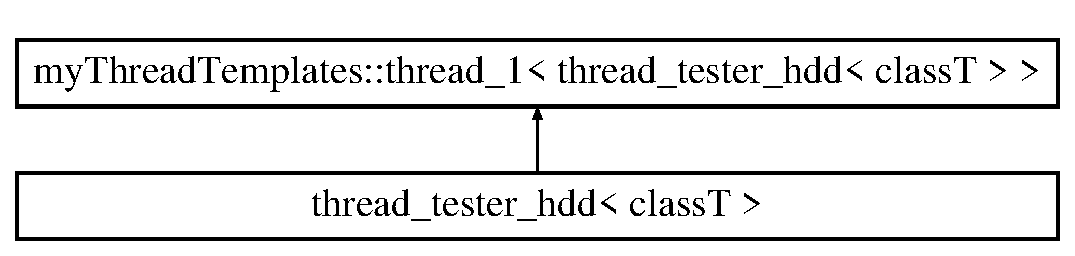
\includegraphics[height=2cm]{classthread__tester__hdd}
\end{center}
\end{figure}
\subsection*{Public Member Functions}
\begin{DoxyCompactItemize}
\item 
\hypertarget{classthread__tester__hdd_ab318188f613c5b36e107084a8229f823}{
\hyperlink{classthread__tester__hdd_ab318188f613c5b36e107084a8229f823}{thread\_\-tester\_\-hdd} (vector$<$ unsigned int $>$, string, string, unsigned int, unsigned int, uint8\_\-t, mode\_\-t, bool)}
\label{classthread__tester__hdd_ab318188f613c5b36e107084a8229f823}

\begin{DoxyCompactList}\small\item\em Headers. \item\end{DoxyCompactList}\item 
\hypertarget{classthread__tester__hdd_ab630709c819674b3eed419e96125d5f1}{
void {\bfseries setNewData} (vector$<$ unsigned int $>$, string)}
\label{classthread__tester__hdd_ab630709c819674b3eed419e96125d5f1}

\item 
\hypertarget{classthread__tester__hdd_a56a89f631010469f197daa1375a4709f}{
void {\bfseries setBuffer} (const unsigned int $\ast$)}
\label{classthread__tester__hdd_a56a89f631010469f197daa1375a4709f}

\item 
\hypertarget{classthread__tester__hdd_a4dff9184fba9308a5803c297c349d075}{
string \& {\bfseries getSummary} ()}
\label{classthread__tester__hdd_a4dff9184fba9308a5803c297c349d075}

\item 
void \hyperlink{classthread__tester__hdd_a9d9f6f67783301bb7d1b9859ecd932c0}{Execute} ()
\end{DoxyCompactItemize}


\subsection{Detailed Description}
Globals Varuabels. 

\subsection{Member Function Documentation}
\hypertarget{classthread__tester__hdd_a9d9f6f67783301bb7d1b9859ecd932c0}{
\index{thread\_\-tester\_\-hdd@{thread\_\-tester\_\-hdd}!Execute@{Execute}}
\index{Execute@{Execute}!thread_tester_hdd@{thread\_\-tester\_\-hdd}}
\subsubsection[{Execute}]{\setlength{\rightskip}{0pt plus 5cm}void thread\_\-tester\_\-hdd::Execute ()}}
\label{classthread__tester__hdd_a9d9f6f67783301bb7d1b9859ecd932c0}


Write test

Both read test

Cleaning after rw tests 



The documentation for this class was generated from the following files:\begin{DoxyCompactItemize}
\item 
thread\_\-tester\_\-hdd.hpp\item 
thread\_\-tester\_\-hdd.cpp\end{DoxyCompactItemize}

\printindex
\end{document}
